\documentclass[a4paper]{article}

  \usepackage{fullpage} % Package to use full page
  \usepackage{parskip} % Package to tweak paragraph skipping
  \usepackage{tikz} % Package for drawing
  \usepackage{tkz-graph}
  \usepackage{amsmath}
  \usepackage{siunitx} % Package for scientific units
  \usepackage{amsfonts}
  \usepackage{amssymb}
  \usepackage{hyperref}
  \usepackage[utf8]{inputenc}
  \usepackage[english]{babel}
  \usepackage{multicol}
  \usepackage{graphicx} % Package for including images
  \graphicspath{ {./images/} }
  
  \DeclareUnicodeCharacter{2212}{-}
  \newcommand\tab[1][0.5cm]{\hspace*{#1}}
  
  \title{Homework 1}
  \author{Adrian Darian}
  \date{9/15/2020}
  
  \begin{document}
  
\maketitle
  
\section*{Chapter 2}
\begin{itemize}
	\item[43] Let $A$ and $B$ be two stations attempting to transmit on an Ethernet. Each has a steady queue of frames ready to send; $A$’s frames will be numbered $A_{1}$, $A_{2}$, and so on, and $B$’s similarly. Let $T = 51.2μs$ be the exponential backoff base unit. Suppose $A$ and $B$ simultaneously attempt to send frame $1$, collide, and happen to choose backoff times of $0 \times T$ and $1 \times T$, respectively, meaning $A$ wins the race and transmits $A_{1}$ while $B$ waits. At the end of this transmission, $B$ will attempt to retransmit $B_{1}$ while $A$ will attempt to transmit $A_{2}$. These first attempts will collide, but now $A$ backs off for either $0 \times T$ or $1 \times T$, while $B$ backs off for time equal to one of $0 \times T, . . . ,3 \times T$.
	      \begin{itemize}
	      	\item[(a)] Give the probability that $A$ wins this second backoff race immediately after this first collision; that is, $A$’s first choice of backoff time $k \times 51.2$ is less than $B$’s. \\
	      	      \textbf{Answer:}  $P(k_{A}, k{B}) = (0, 1)(0, 2)(0, 3)(1, 2)(1, 3) = \frac{5}{8}$ \\
	      	      $\therefore count(k_{A}) + count(k_{B}) / count(k_{A}) \times count(k_{B}) = \frac{5}{8}$
	      	\item[(b)] Suppose $A$ wins this second backoff race. $A$ transmits $A_{3}$, and when it is finished, $A$ and $B$ collide again as $A$ tries to transmit $A_{4}$ and $B$ tries once more to transmit $B_{1}$. Give the probability that $A$ wins this third backoff race immediately after the first collision. \\
	      	      \textbf{Answer:} \begin{equation*}
	      	      \begin{cases}
	      	      	k_{B} = 7 of 8 \quad & \text{if} \, k_{A} = 0 \\
	      	      	k_{B} = 6 of 8 \quad & \text{if} \, k_{A} = 1 \\
	      	      \end{cases}
	      	\end{equation*}
	      	$\therefore \frac{7 + 6}{count(k_{A}) \times count(k_{B})} = \frac{13}{16}$
	      	\item[(c)] Give a reasonable lower bound for the probability that $A$ wins all the remaining backoff races. \\
	      	      \textbf{Answer:} Since the probabilities of $A$ winning race $1$ and $2$ with $\frac{5}{8}$ and $\frac{13}{16}$ respectively, we can grab a lower bound for each of $\frac{1}{2}$ and $\frac{3}{4}$. A generalized equation to recreate this event would be $(1 - \frac{1}{2^{i - 1}})$, where $A$ wins all $3$ of the initial races.
	      	\item[(d)] What then happens to the frame $B_{1}$? This scenario is known as the Ethernet capture effect. \\
	      	      \textbf{Answer:} It just starts all over again but at $B_{2}$ this time.
	      \end{itemize}
	\item[53] How can a wireless node interfere with the communications of another node when the two nodes are separated by a distance greater than the transmission range of either node? \\
	      \textbf{Answer:} We have $2$ communicaton connections: $A -> B$ and $C -> B$. Wireless interferance would occur when node $C$ interferes with the $A -> B$ connection and where $A$ interferes with the $C -> B$ connection.
	\item[55] How can hidden terminals be detected in $802.11$ networks? \\
	      \textbf{Answer:} First you send off a RTS (Request to Send) packet. Then the receiver sends a reply as a CTS (Cleared to Send) packet. The second the initial transmitter gets the CTS from the receiver it send the data packets. There is a case though that if the transmitter never receives the encoded duration field that is within the CTS then the transmitter will enter a backoff mode. 
\end{itemize}

\section*{Chapter 3}
\begin{itemize}
	\item[3] For the network given in Figure 3.45, give the datagram forwarding table for each node. The links are labeled with relative costs; yourtables should forward each packet via the lowest-cost path to its destination \\
	      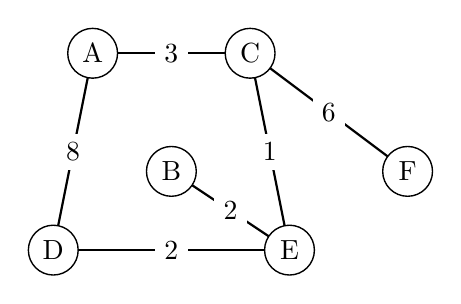
\begin{tikzpicture}
	      	\Vertex[x = 0,    y = 0]{B}
	      	\Vertex[x = 1,    y = 1.5]{C}
	      	\Vertex[x = 1.5,  y = -1]{E}
	      	\Vertex[x = -1.5, y = -1]{D}
	      	\Vertex[x = -1,   y = 1.5]{A}
	      	\Vertex[x = 3,    y = 0]{F}
	      	\Edge[label = $2$](B)(E)
	      	\Edge[label = $2$](E)(D)
	      	\Edge[label = $8$](D)(A)
	      	\Edge[label = $3$](A)(C)
	      	\Edge[label = $1$](C)(E)
	      	\Edge[label = $6$](C)(F)
	      \end{tikzpicture}  \\
	      \textbf{Answer:} \\
	      Node A: \begin{tabular}{c|c}
	      Destination & Hop \\
	      B & C \\
	      C & C \\
	      D & C \\
	      E & C \\
	      F & C \\
	\end{tabular}
	Node B: \begin{tabular}{c|c}
	Destination & Hop \\
	A & E \\
	C & E \\
	D & E \\
	E & E \\
	F & E \\
	\end{tabular}
	Node C: \begin{tabular}{c|c}
	Destination & Hop \\
	A & A \\
	B & E \\
	D & E \\
	E & E \\
	F & F \\
	\end{tabular} \\
	Node D: \begin{tabular}{c|c}
	Destination & Hop \\
	A & E \\
	B & E \\
	C & E \\
	E & E \\
	F & E \\
	\end{tabular}
	Node E: \begin{tabular}{c|c}
	Destination & Hop \\
	A & C \\
	B & B \\
	C & C \\
	D & D \\
	F & C \\
	\end{tabular}
	Node F: \begin{tabular}{c|c}
	Destination & Hop \\
	A & C \\
	B & C \\
	C & C \\
	D & C \\
	E & C \\
	\end{tabular}
	\item[13] Given the extended LAN shown in Figure 3.48, indicate which ports are not selected by the spanning tree algorithm. \\
	      \textbf{Answer:} \\
	      \begin{tabular}{c c c c}
	      	B1: & (B1, B1, 0) & (B1, B1, 0) & (B1, B1, 0) \\
	      	B2: & (B2, B2, 0) & (B2, B2, 0) & (B2, B1, 2) \\
	      	B3: & (B3, B3, 0) & (B3, B1, 1) & (B3, B1, 1) \\
	      	B4: & (B4, B4, 0) & (B4, B1, 2) & (B4, B1, 2) \\
	      	B5: & (B5, B5, 0) & (B5, B2, 1) & (B5, B1, 2) \\
	      	B6: & (B6, B6, 0) & (B6, B1, 2) & (B6, B1, 2) \\
	      	B7: & (B7, B7, 0) & (B7, B1, 1) & (B7, B1, 1) \\
	      \end{tabular}
	\item[15] Consider the arrangement of learning bridges shown in Figure 3.49. Asusming all are initially empty, give the forwarding tables for each of the bridges B1 to B4 after the following transmissions: \\
	      \begin{itemize}
	      	\item A sends to C.
	      	\item C sends to A.
	      	\item D sends to C.
	      \end{itemize}
	      Identify ports with the unique neighbor reached directly from that port; that is, the ports for B1 are to be labeled "A" and "B2". \\
	      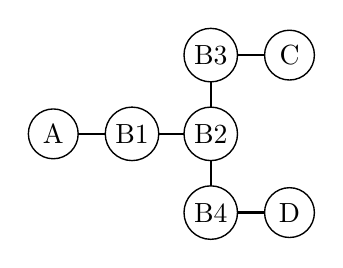
\begin{tikzpicture}
	      	\Vertex[x = 0, y = 0]{B2}
	      	\Vertex[x = -1, y = 0]{B1}
	      	\Vertex[x = -2, y = 0]{A}
	      	\Vertex[x = 0, y = 1]{B3}
	      	\Vertex[x = 1, y = 1]{C}
	      	\Vertex[x = 0, y = -1]{B4}
	      	\Vertex[x = 1, y = -1]{D}
	      	\Edge[](B2)(B1)
	      	\Edge[](B2)(B3)
	      	\Edge[](B2)(B4)
	      	\Edge[](B1)(A)
	      	\Edge[](B3)(C)
	      	\Edge[](B4)(D)
	      \end{tikzpicture} \\
	      \textbf{Answer:} \\
	      \begin{tabular}{c c c c c c}
	      	B1: & (A, A)        & (B2, C) &         \\
	      	B2: & (B1, A)       & (B3, C) & (B4, D) \\
	      	B3: & (B2, A and D) & (C, C)  &         \\
	      	B4: & (B2, A)       & (D, D)  &         \\
	      \end{tabular}
	\item[17] Consider hosts X, Y, Z, W and learning bridges B1, B2, B3, with initially empty forwarding tables, as in Figure 3.50.
	      \begin{itemize}
	      	\item[(a)] Suppose X sends to W. Which Bridges learn where X is? Does Y's network interface see this packet? \\
	      	      \textbf{Answer:} Because the path from X to W passes through all bridges each node in the network knows of the location of X.
	      	\item[(b)] Suppose Z now sends to X. Which bridges learn where Z is? Does Y's network interface see this packet? \\
	      	      \textbf{Answer:} Because X's location is already known the packet is sent directly to X from Z and Y is never reached because B2 immediately sends to B1
	      	\item[(c)] Suppose Y now sends to X. Which bridges learn where Y is? Does Z's network interface see this packet? \\
	      	      \textbf{Answer:} Because the only connection to Y is B2 and B2 knows that to the left is B1 and then X it just sends straight from Y to B2 to B1 to X. Never informing B3 or Z
	      	\item[(d)] Finally, suppose W sends to Y. Which bridges learn where W is? Does Z's network interface see this packet? \\
	      	      \textbf{Answer:} Because B3 never interacted with Y it has to push the packet to Z instead, luckily Z knows where Y is but once it gets there, B1 was never informed of the packet, meaning that B1 does not know where Y is.
	      \end{itemize} 
	      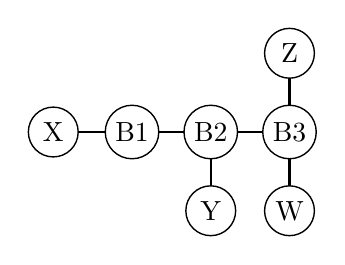
\begin{tikzpicture}
	      	\Vertex[x = 0, y = 0]{X}
	      	\Vertex[x = 1, y = 0]{B1}
	      	\Vertex[x = 2, y = 0]{B2}
	      	\Vertex[x = 2, y = -1]{Y}
	      	\Vertex[x = 3, y = 0]{B3}
	      	\Vertex[x = 3, y = 1]{Z}
	      	\Vertex[x = 3, y = -1]{W}
	      	\Edge[](X)(B1)
	      	\Edge[](B1)(B2)
	      	\Edge[](B2)(Y)
	      	\Edge[](B2)(B3)
	      	\Edge[](B3)(Z)
	      	\Edge[](B3)(W)
	      \end{tikzpicture}
	\item[33] What aspect of IP address makes it necessary to have one address per network interface, rather than just one per host? In light of your answer, why does IP tolerate point-to-point interfaces that have nonunique addresses or no addresses? \\
	      \textbf{Answer:} The subnet, because point-to-point allows duplicate addresses
	\item[36] Suppose a TCP message that contains 1024 bytes of data and 20 bytes of TCP header is passed to IP for delivery across two networks interconnected by a router (i.e., it travels from the source host to a router to the destination host). The first network has an MTU of 1024 bytes; the second has an MTU of 576 bytes. Each network’s MTU gives the size of the largest IP datagram that can be carried in a link-layer frame. Give the sizes and offsets of the sequence of fragments delivered to the network layer at the destination host. Assume all IP headers are 20 bytes. \\
	      \textbf{Answer:} \\
	      \begin{tabular}{r c l}
	      	First MTU                   &     &        \\
	      	$1024 - 20$                 & $=$ & $1004$ \\
	      	$8 \times [\frac{1004}{8}]$ & $=$ & $1000$ \\
	      	$1024 + 20$                 & $=$ & $1044$ \\
	      	Second MTU                  &     &        \\
	      	$576 - 20$                  & $=$ & $556$  \\
	      	$8 \times [\frac{556}{8}]$  & $=$ & $552$  \\
	      \end{tabular}
	\item[46] For the network shown in Figure 3.53, give global distance-vector tables like those of Tables 3.10 and 3.13 when
	      \begin{itemize}
	      	\item[(a)] Each node knows only the distances to its immediate neighbors. \\
	      	      \textbf{Answer:} \\
	      	      \begin{tabular}{|c|c|c|c|c|c|c|}
	      	      	\hline
	      	      	  & A & B & C & D & E & F \\
	      	      	\hline
	      	      	A & 0 &   & 3 & 8 &   &   \\
	      	      	B &   & 0 &   &   & 2 &   \\
	      	      	C & 3 &   & 0 &   & 1 & 6 \\
	      	      	D & 8 &   &   & 0 & 2 &   \\
	      	      	E &   & 2 & 1 & 2 & 0 &   \\
	      	      	F &   &   & 6 &   &   & 0 \\
	      	      	\hline						
	      	      \end{tabular}
	      	\item[(b)] Each node has reported the information it had in the preceding step to its immediate neighbors. \\
	      	      \textbf{Answer:} \\
	      	      \begin{tabular}{|c|c|c|c|c|c|c|}
	      	      	\hline
	      	      	  & A & B & C & D & E & F \\
	      	      	\hline
	      	      	A & 0 &   & 3 & 8 & 4 & 9 \\
	      	      	B &   & 0 & 3 & 4 & 2 &   \\
	      	      	C & 3 & 3 & 0 & 3 & 1 & 6 \\
	      	      	D & 8 & 4 & 3 & 0 & 2 &   \\
	      	      	E & 4 & 2 & 1 & 2 & 0 & 7 \\
	      	      	F & 9 &   & 6 &   & 7 & 0 \\
	      	      	\hline						
	      	      \end{tabular}
	      	\item[(c)] Step (b) happens a second time. \\
	      	      \textbf{Answer:} \\
	      	      \begin{tabular}{|c|c|c|c|c|c|c|}
	      	      	\hline
	      	      	  & A & B & C & D & E & F \\
	      	      	\hline
	      	      	A & 0 & 6 & 3 & 6 & 4 & 9 \\
	      	      	B & 6 & 0 & 3 & 4 & 2 & 9 \\
	      	      	C & 3 & 3 & 0 & 3 & 1 & 6 \\
	      	      	D & 6 & 4 & 3 & 0 & 2 & 9 \\
	      	      	E & 4 & 2 & 1 & 2 & 0 & 7 \\
	      	      	F & 9 & 9 & 6 & 9 & 7 & 0 \\
	      	      	\hline						
	      	      \end{tabular}
	      \end{itemize} 
	      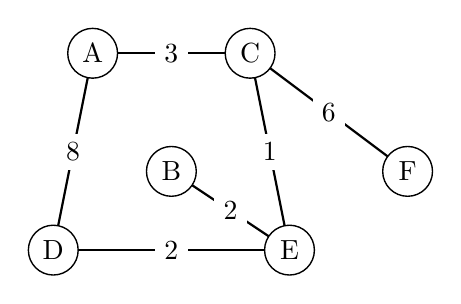
\begin{tikzpicture}
	      	\Vertex[x = 0,    y = 0]{B}
	      	\Vertex[x = 1,    y = 1.5]{C}
	      	\Vertex[x = 1.5,  y = -1]{E}
	      	\Vertex[x = -1.5, y = -1]{D}
	      	\Vertex[x = -1,   y = 1.5]{A}
	      	\Vertex[x = 3,    y = 0]{F}
	      	\Edge[label = $2$](B)(E)
	      	\Edge[label = $2$](E)(D)
	      	\Edge[label = $8$](D)(A)
	      	\Edge[label = $3$](A)(C)
	      	\Edge[label = $1$](C)(E)
	      	\Edge[label = $6$](C)(F)
	      \end{tikzpicture} 
	\item[48] For the network given in Figure 3.53, show how the link-state algorithm builds the routing table for node D. \\
	      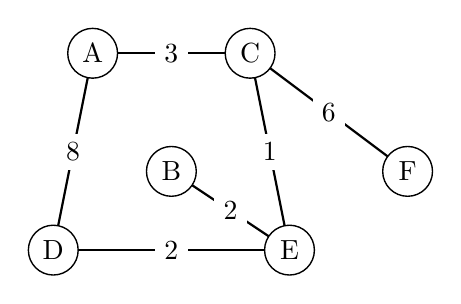
\begin{tikzpicture}
	      	\Vertex[x = 0,    y = 0]{B}
	      	\Vertex[x = 1,    y = 1.5]{C}
	      	\Vertex[x = 1.5,  y = -1]{E}
	      	\Vertex[x = -1.5, y = -1]{D}
	      	\Vertex[x = -1,   y = 1.5]{A}
	      	\Vertex[x = 3,    y = 0]{F}
	      	\Edge[label = $2$](B)(E)
	      	\Edge[label = $2$](E)(D)
	      	\Edge[label = $8$](D)(A)
	      	\Edge[label = $3$](A)(C)
	      	\Edge[label = $1$](C)(E)
	      	\Edge[label = $6$](C)(F)
	      \end{tikzpicture} 	  
	      \textbf{Answer:} \\
	      %   \scalebox{0.8}{
	      \begin{tabular}{cll}
	      	  & Confirmed                                                   & Tentative                     \\
	      	1 & (D, 0, -)                                                   &                               \\
	      	2 & (D, 0, -)                                                   & (A, 8, A) (E, 2, E)           \\
	      	3 & (D, 0, -) (E, 2, E)                                         & (A, 8, A) (B, 4, E) (C, 3, E) \\
	      	4 & (D, 0, -) (E, 2, E) (C, 3, E)                               & (A, 6, E) (B, 4, E) (F, 9, E) \\
	      	5 & (D, 0, -) (E, 2, E) (C, 3, E) (B, 4, E)                     & (A, 6, E) (F, 9, E)           \\
	      	6 & (D, 0, -) (E, 2, E) (C, 3, E) (B, 4, E) (A, 6, E)           &                               \\
	      	7 & (D, 0, -) (E, 2, E) (C, 3, E) (B, 4, E) (A, 6, E) (F, 9, E) &                               \\
	      \end{tabular}
	      %   }
	\item[54] For the network in Figure 3.53, suppose the forwarding tables are all established as in Exercise 46 and then the C-E link fails. Give:
	      \begin{itemize}
	      	\item[(a)] The tables of A, B, D, and F after C and E have reported the news. \\
	      	      \textbf{Answer:} \\
	      	      Node A: \begin{tabular}{c|c|c}
	      	      destination & cost & hop \\
	      	      \hline
	      	      B & & - \\
	      	      C & 3 & C \\
	      	      D & & - \\
	      	      E & & - \\
	      	      F & 9 & C \\
	      	\end{tabular}
	      	Node B: \begin{tabular}{c|c|c}
	      	destination & cost & hop \\
	      	\hline
	      	A &   & - \\
	      	C &   & - \\
	      	D & 4 & E \\
	      	E & 3 & E \\
	      	F &   & - \\
	      	\end{tabular}
	      	Node D: \begin{tabular}{c|c|c}
	      	destination & cost & hop \\
	      	\hline
	      	A &   & - \\
	      	B & 4 & E \\
	      	C &   & - \\
	      	E & 2 & E \\
	      	F &   & - \\
	      	\end{tabular}
	      	Node F: \begin{tabular}{c|c|c}
	      	destination & cost & hop \\
	      	\hline
	      	A & 9 & C \\
	      	B &   & - \\
	      	C & 6 & C \\
	      	D &   & - \\
	      	E &   & - \\
	      	\end{tabular}
	      	\item[(b)] The tables of A and D after their next mutual exchange. \\
	      	      \textbf{Answer:} \\
	      	      Node A: \begin{tabular}{c|c|c}
	      	      destination & cost & hop \\
	      	      \hline
	      	      B & 12 & D \\
	      	      C & 3  & C \\
	      	      D & 8  & D \\
	      	      E & 10 & D \\
	      	      F & 9  & C \\
	      	\end{tabular}
	      	Node D: \begin{tabular}{c|c|c}
	      	destination & cost & hop \\
	      	\hline
	      	A & 8  & A \\
	      	B & 4  & E \\
	      	C & 11 & A \\
	      	E & 2  & E \\
	      	F & 17 & A \\
	      	\end{tabular}
	      	\item[(c)] The table of C after A exchanges with it. \\
	      	      \textbf{Answer:} \\
	      	      Node C: \begin{tabular}{c|c|c}
	      	      destination & cost & hop \\
	      	      \hline
	      	      A & 3  & A \\
	      	      B & 15 & A \\
	      	      D & 11 & A \\
	      	      E & 13 & A \\
	      	      F & 6  & F \\
	      	\end{tabular}
	      \end{itemize} 
	      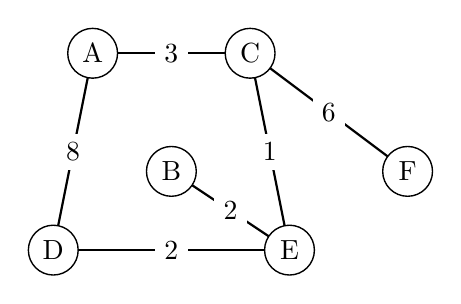
\begin{tikzpicture}
	      	\Vertex[x = 0,    y = 0]{B}
	      	\Vertex[x = 1,    y = 1.5]{C}
	      	\Vertex[x = 1.5,  y = -1]{E}
	      	\Vertex[x = -1.5, y = -1]{D}
	      	\Vertex[x = -1,   y = 1.5]{A}
	      	\Vertex[x = 3,    y = 0]{F}
	      	\Edge[label = $2$](B)(E)
	      	\Edge[label = $2$](E)(D)
	      	\Edge[label = $8$](D)(A)
	      	\Edge[label = $3$](A)(C)
	      	\Edge[label = $1$](C)(E)
	      	\Edge[label = $6$](C)(F)
	      \end{tikzpicture} 
\end{itemize}

\section*{Playing with ping:}

Use the ping command to measure and report the average round trip time between a Linux desktop on the SE1 Linux lab and the following machines:

\begin{itemize}
	\item[(a)] mars.ucmerced.edu \\
	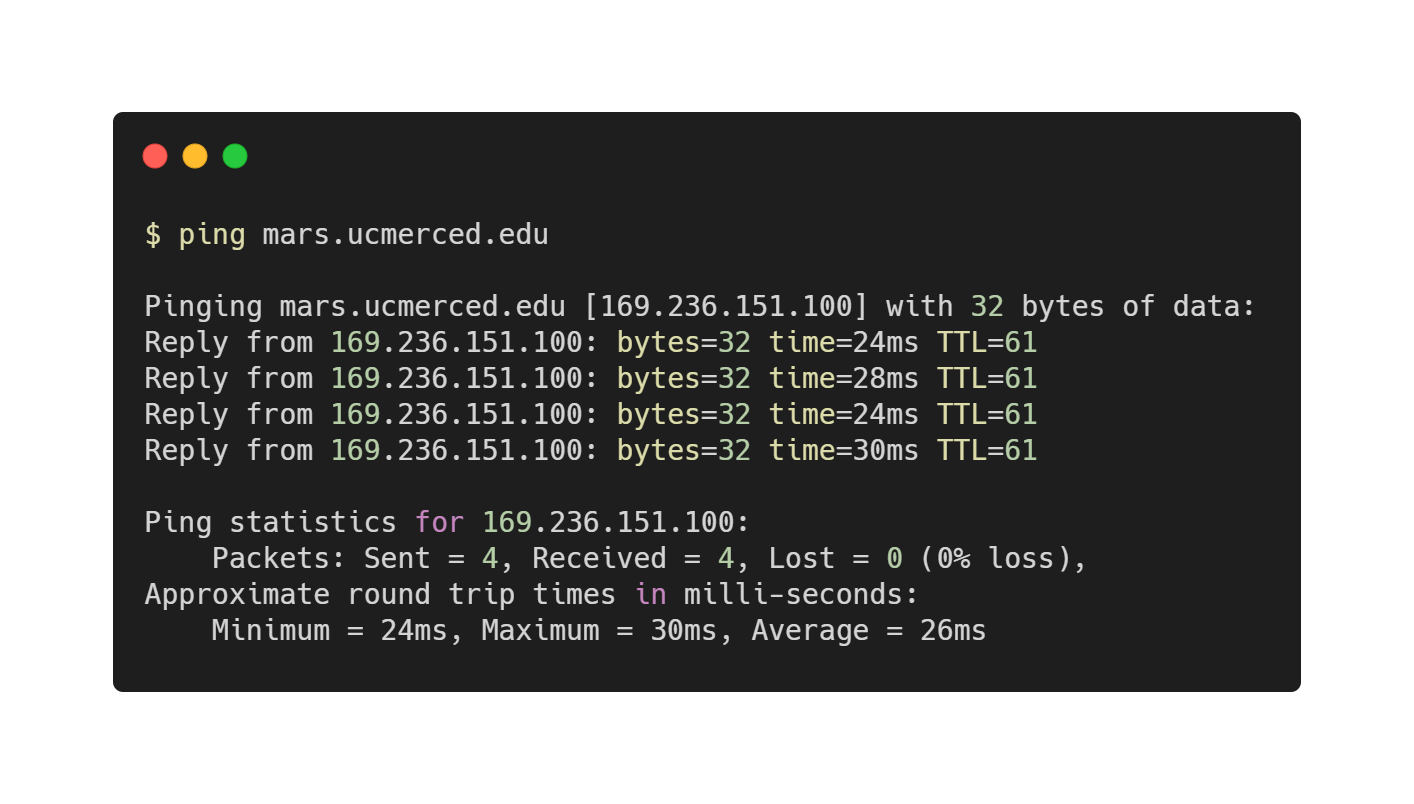
\includegraphics[scale=0.3]{ping-mars.png}
	\item[(b)] www.berkeley.edu \\
	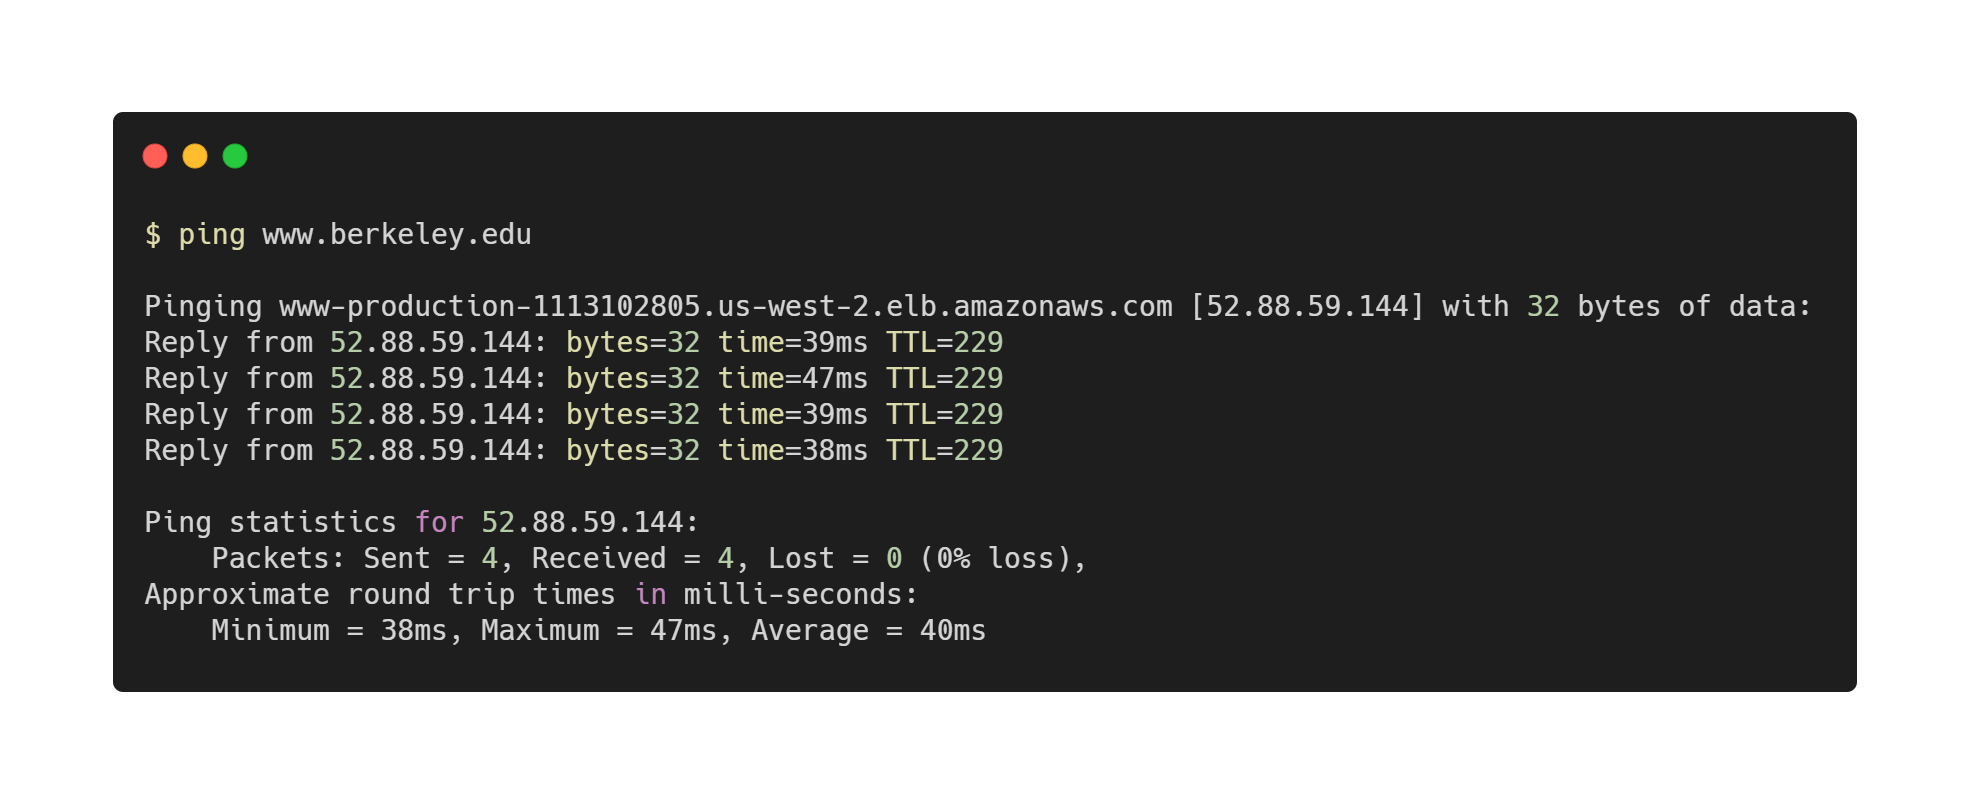
\includegraphics[scale=0.2]{ping-berkeley.png} 
	\item[(c)] www.columbia.edu \\
	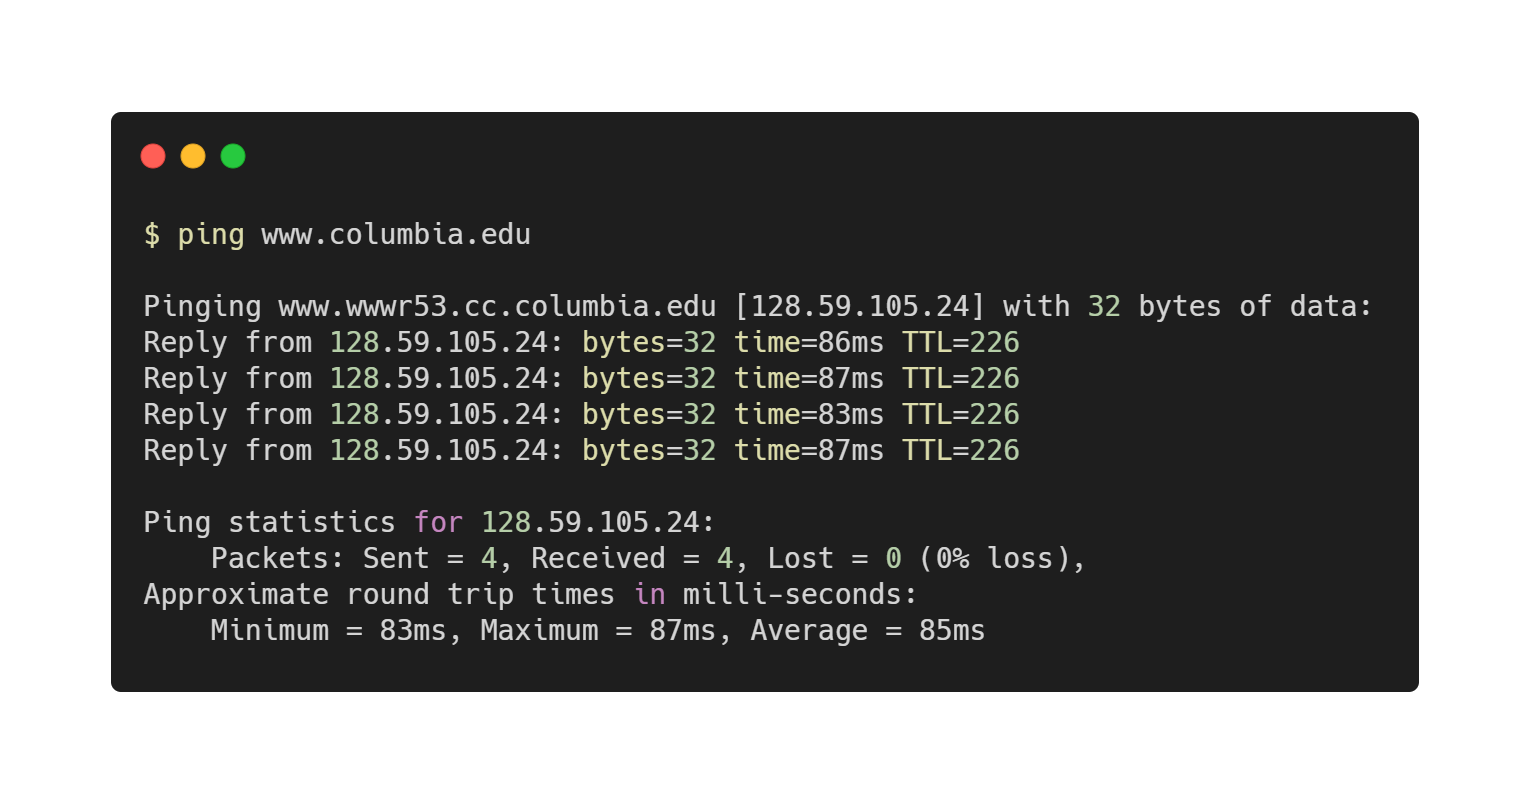
\includegraphics[scale=0.3]{ping-columbia.png} 
	\item[(d)] www.uba.ar \\
	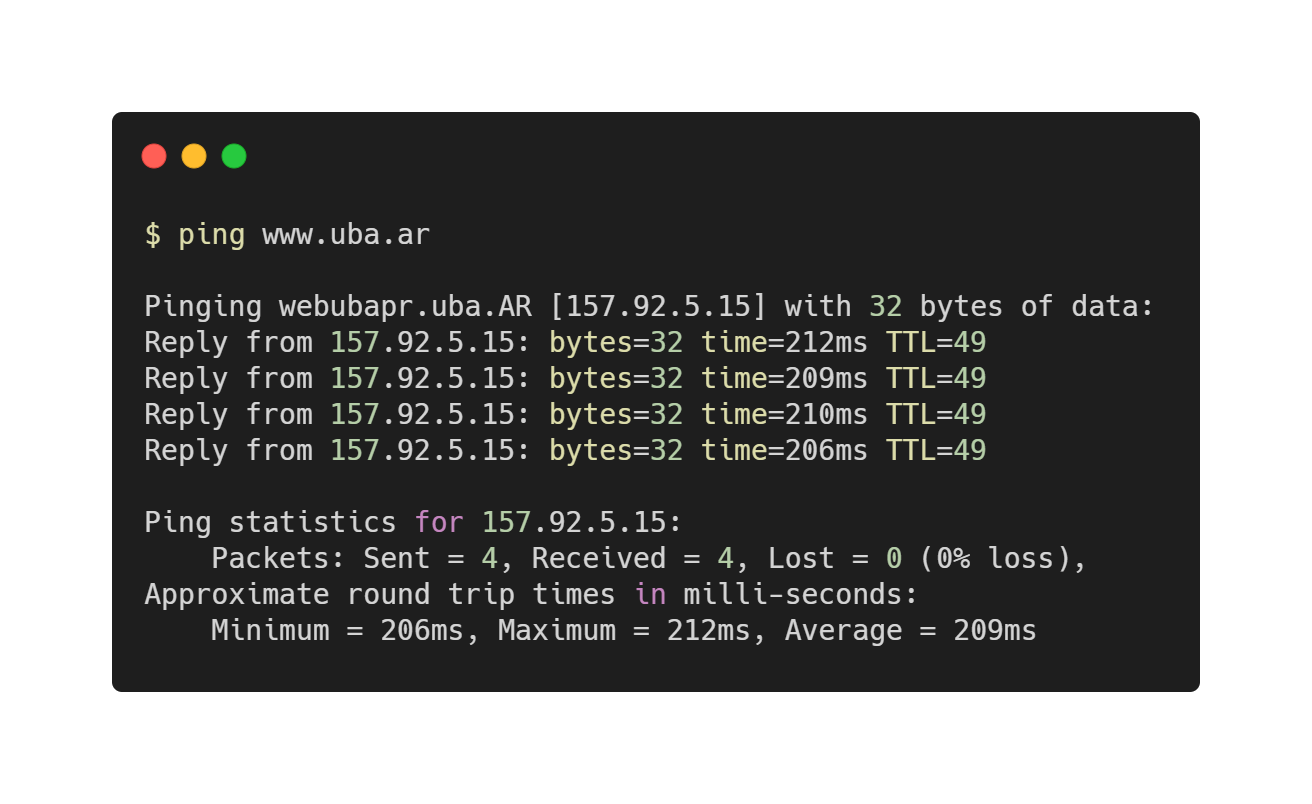
\includegraphics[scale=0.3]{ping-uba.png} 
	\item[(e)] sydney.edu.au \\
	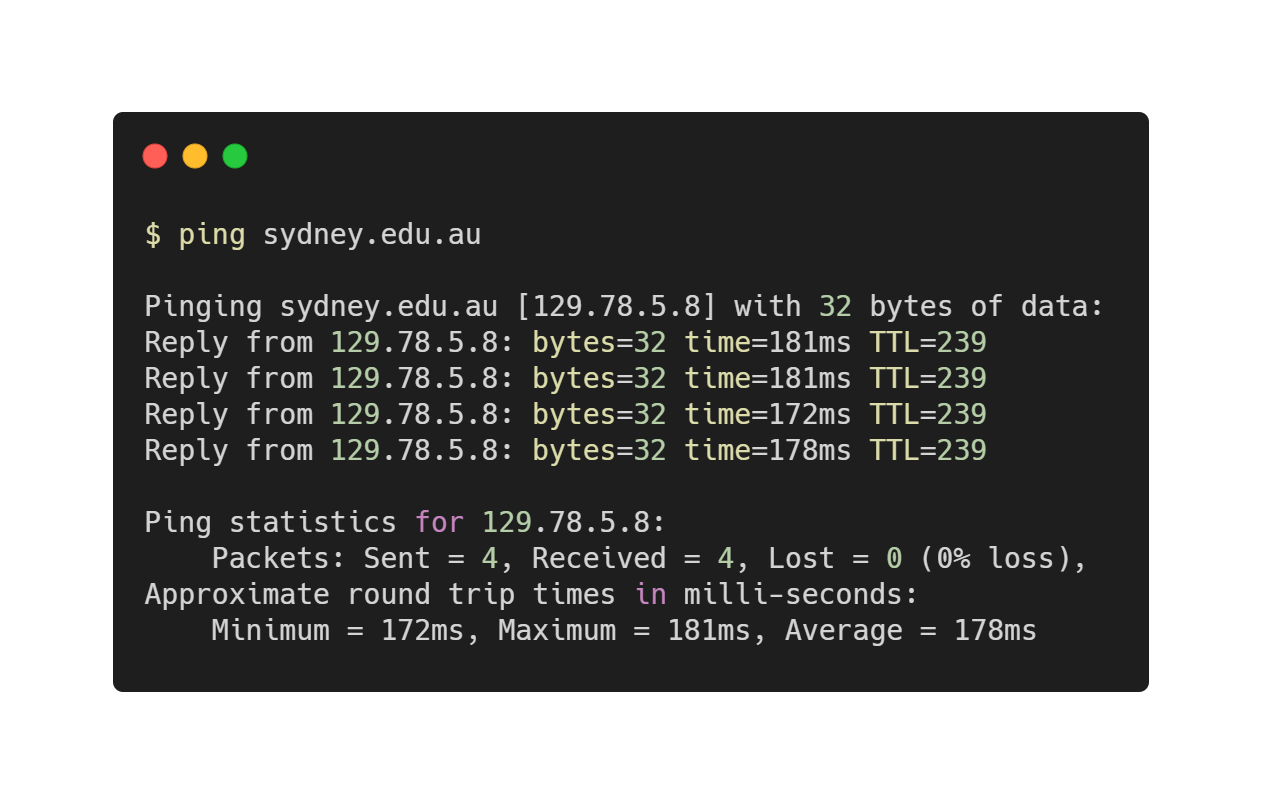
\includegraphics[scale=0.3]{ping-sydney.png} 
\end{itemize}

For each, estimate the physical distance between engineering lab and the destination. Calculate the speed-of-light round-trip delay given this distance. At what fraction of the speed of light did your ping packets travel, for each? \\


\section*{(Bonus extra credit) traceroute problem:}

Use "traceroute" to determine the path taken between a machine in the SE1 lab and 

\begin{itemize}
	\item[(a)] www.uba.ar \\
	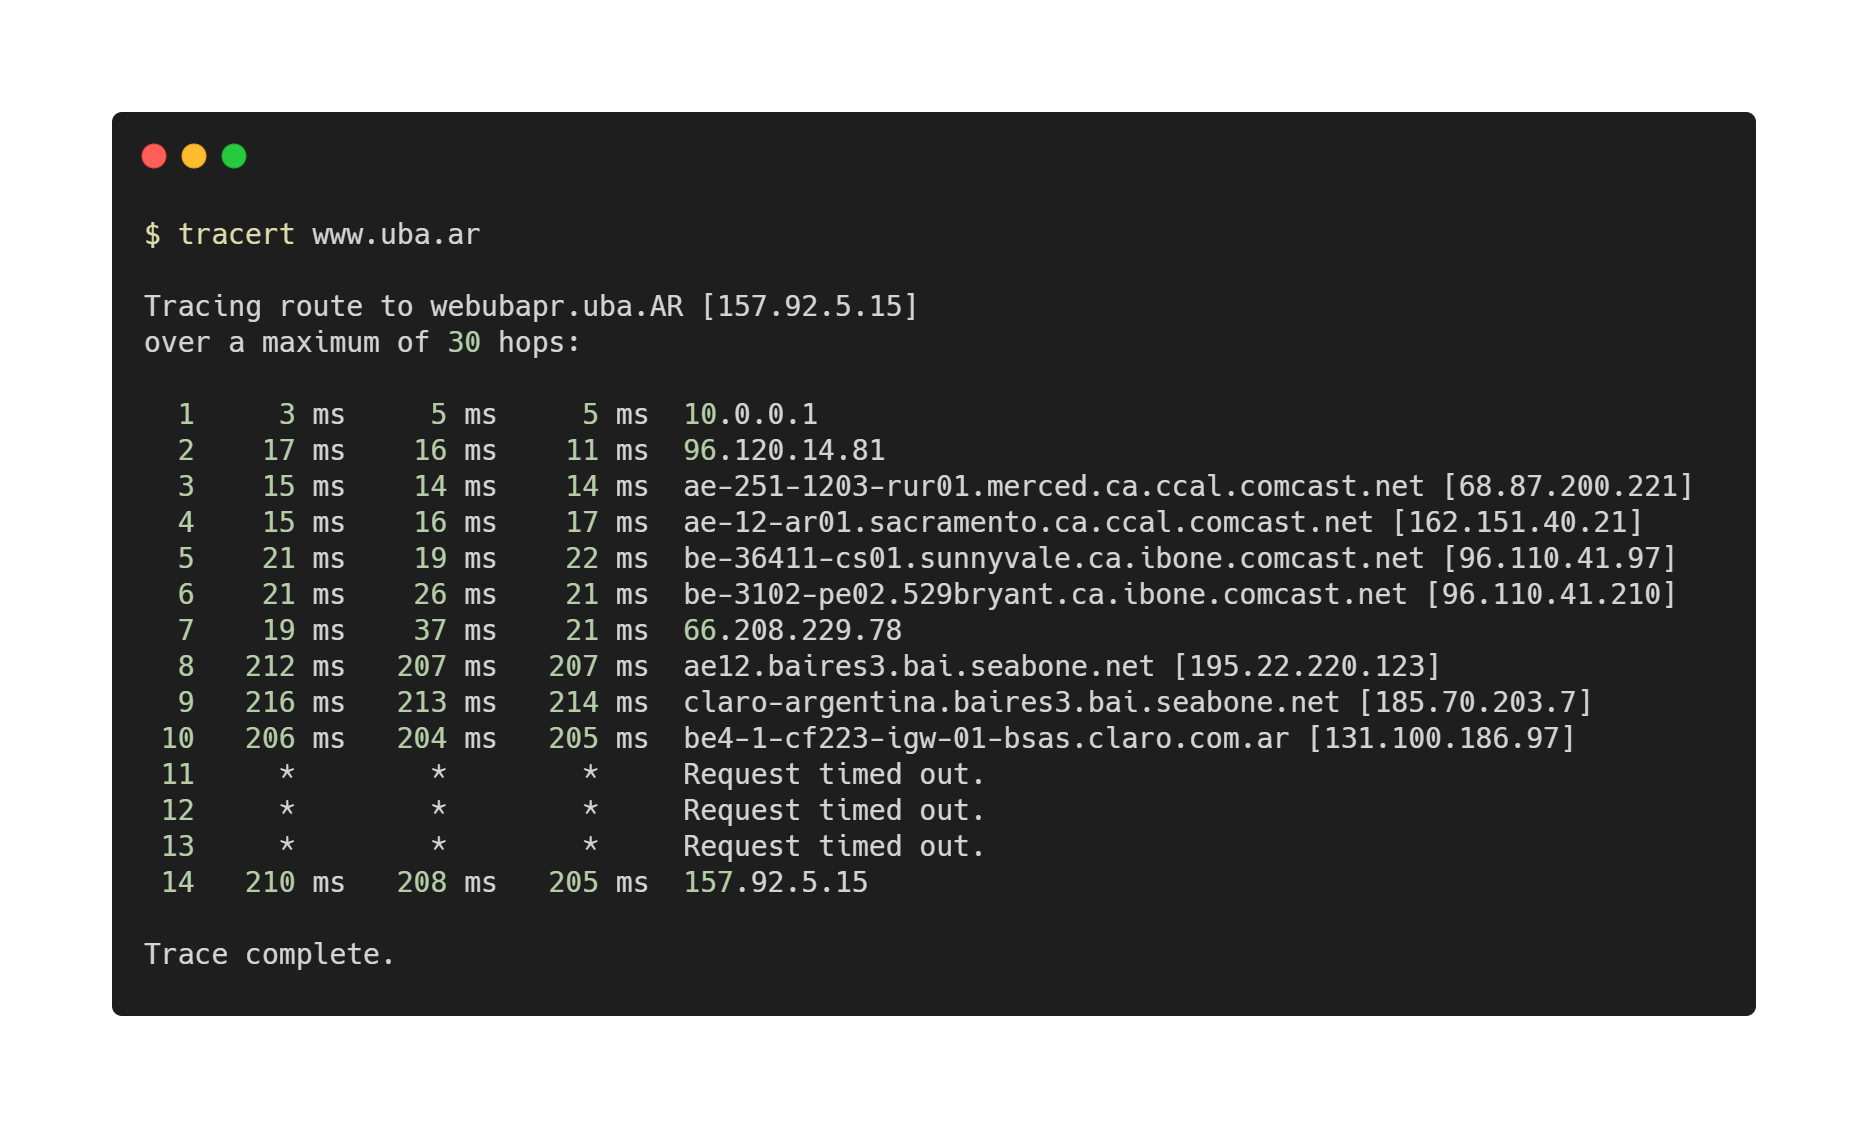
\includegraphics[scale=0.3]{trace-uba.png} 
	\item[(b)] sydney.edu.au \\
	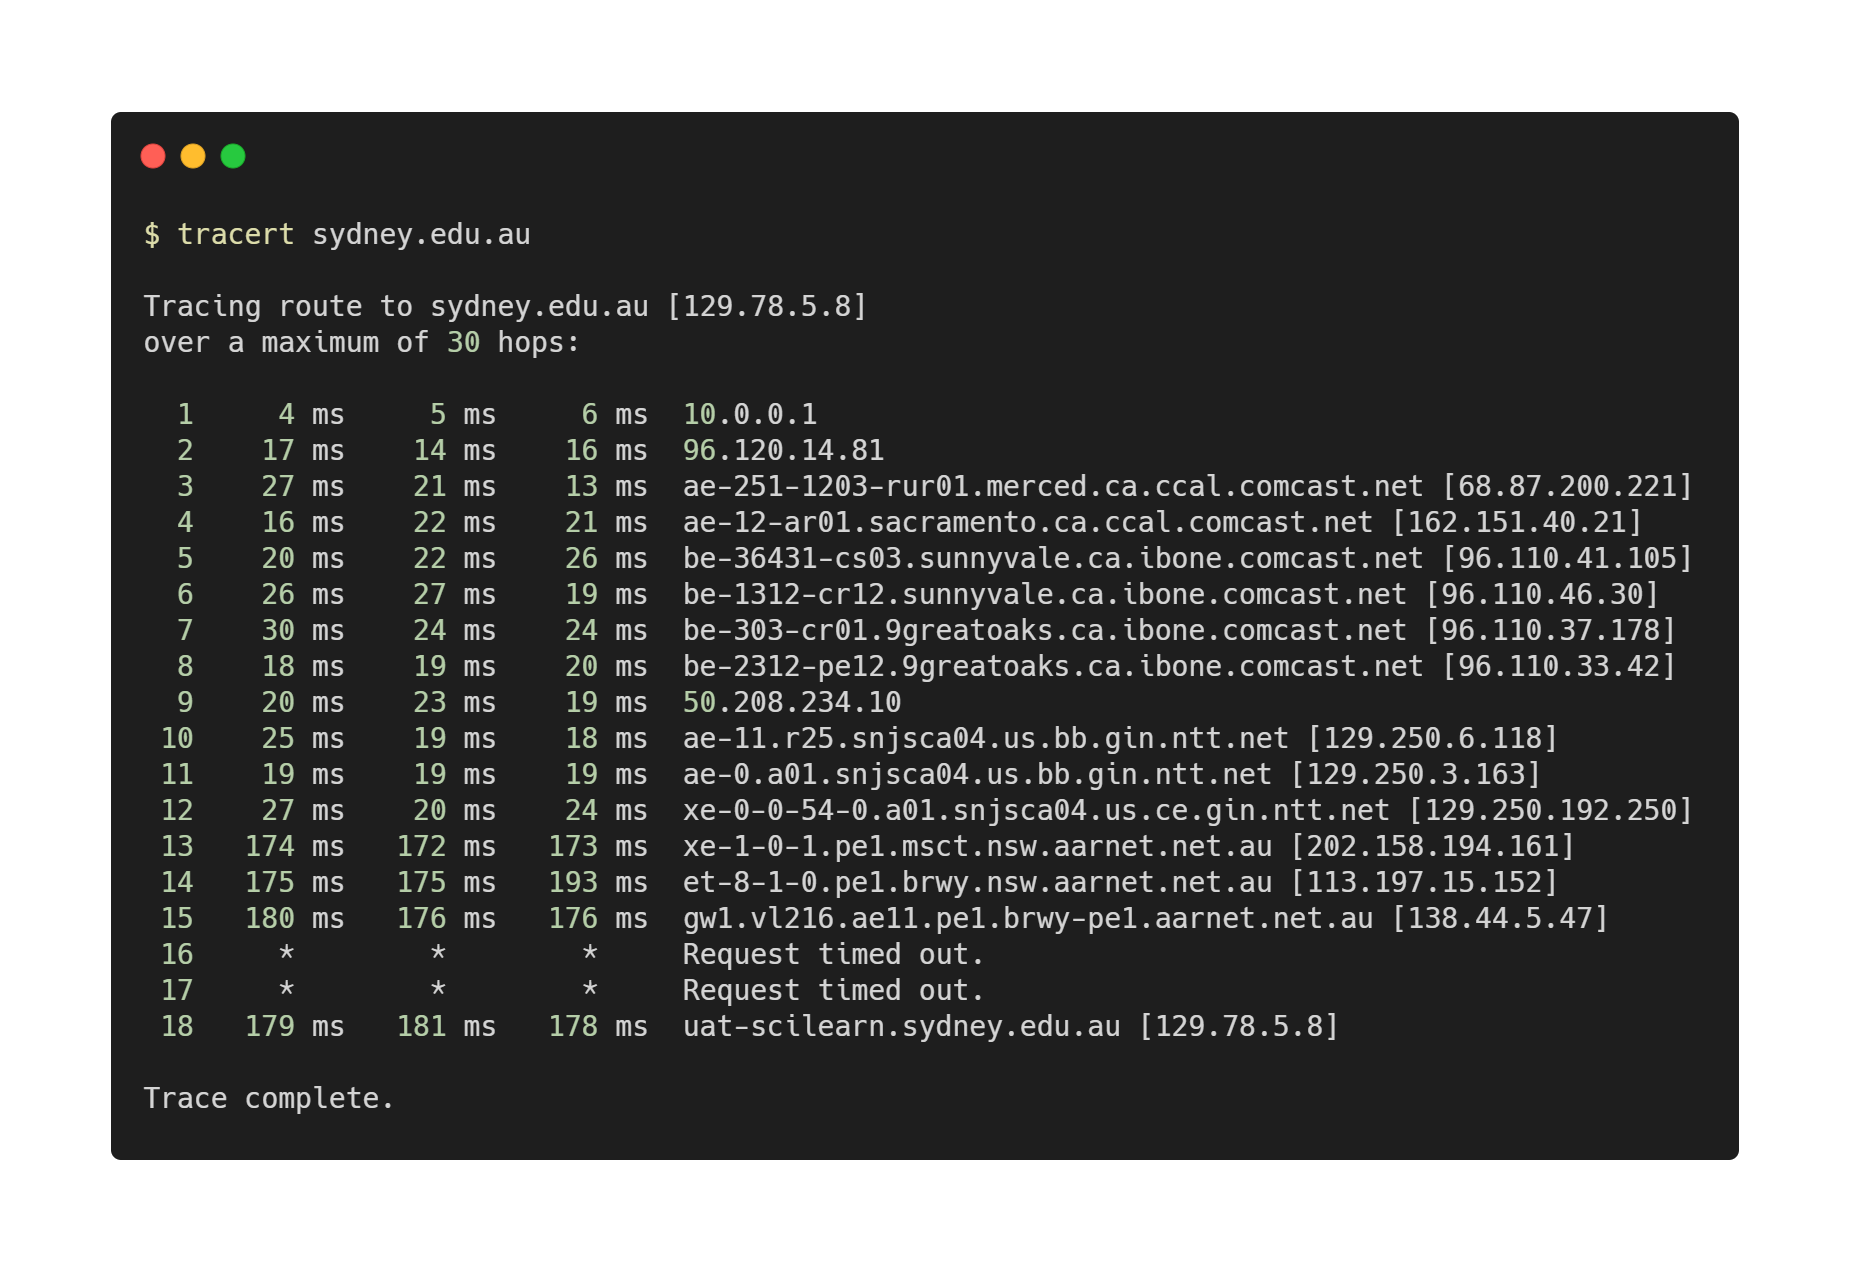
\includegraphics[scale=0.3]{trace-sydney.png} 
\end{itemize}

From its output, using your powers of sleuthing, google, and best guesses, describe the geographical path the packets take -- cities and countries at each hop.

\end{document}